\slide{ Overview }
{
\iteb
\item Academics (2006-2009)
\item FTK: software and simulations (2006-2010)
\item FTK: hardware (2011-2012)
\item ATLAS: daily trigger validation shifts (2012-2013)
\item ATLAS: muon momentum scale (2010-2011)
\item ATLAS: W boson cross-section (2010-2013)
\iteb
\item This is the topic of my Ph.D. thesis
\item Advised by Mel Shochet and Peter Onyisi
\itee
\itee
}

\slide{ 2006-2009: academics }
{
\iteb
\item Took and passed Candidacy Exam in Fall 2007
\item Experimental project: JPARC trigger electronics
\item Post-Candidacy courses
\iteb
\item A: Condensed matter: PHYS361 (Solid State Physics)
\item B: Particle physics: PHYS363 (Particle Physics) and PHYS444 (QFT)
\item C: Large-scale: PHYS372 (Space Physics and Astrophysics)
\item D: Intermediate electives: PHYS386 (Data Analysis)
\item E: Advanced electives: PHYS471 (Atomic) and PHYS491 (Bio)
\itee
\item All formal post-candidacy requirements are satisfied
\itee
}

% LHC
\slide{ The Large Hadron Collider }
{
\centering
LHC: world's largest particle accelerator located at CERN (near Geneva). \\
Designed for pp collisions at 14 TeV, luminosity $\mathcal{O}(10^{34}cm^{-2}s^{-1})$ \\
2012 collision energy (8 TeV) is four times higher than at Tevatron.
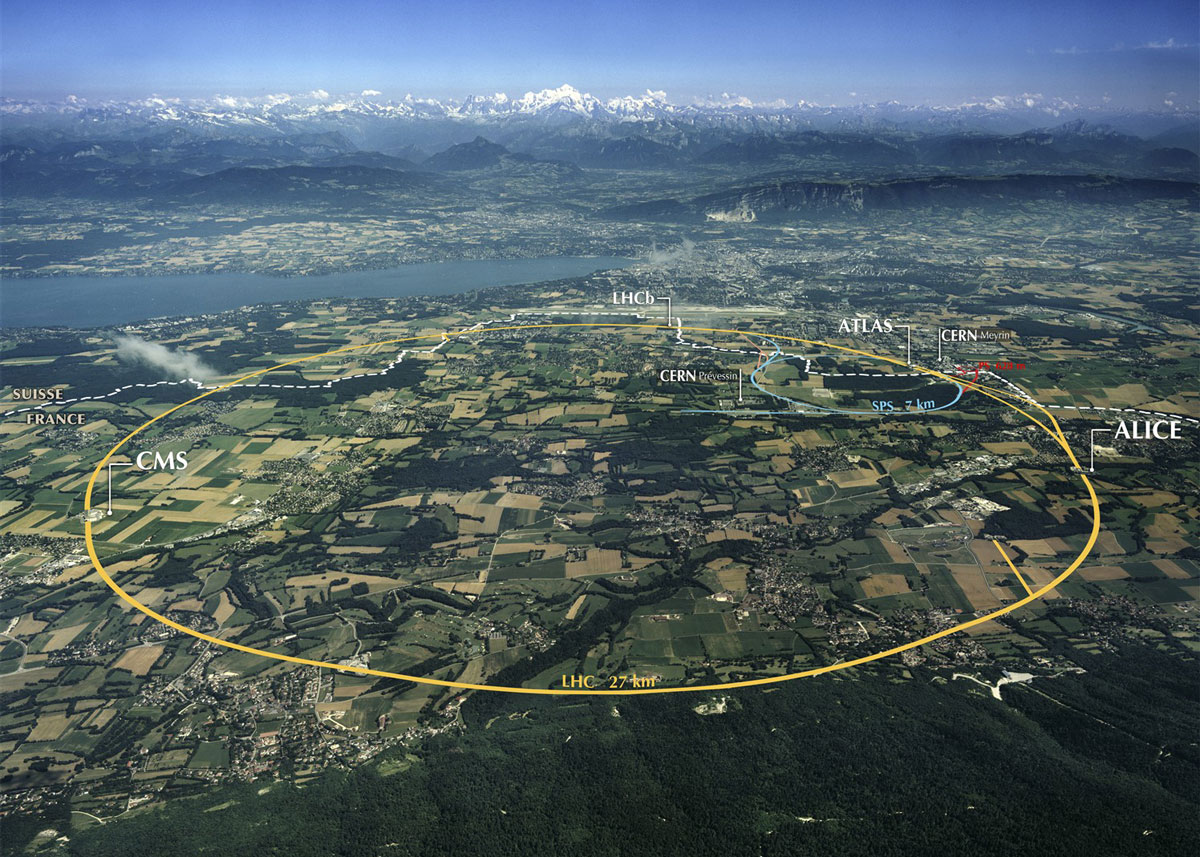
\includegraphics[width=0.8\textwidth]{dates/mtg/figures/atlas/LHC}

}

% ATLAS cavern
\slide{ ATLAS experiment: overview }
{
\centering
One of the two general-purpose experiments at LHC.\\
100 meters underground, 45 meters long, 7000 tons. \\
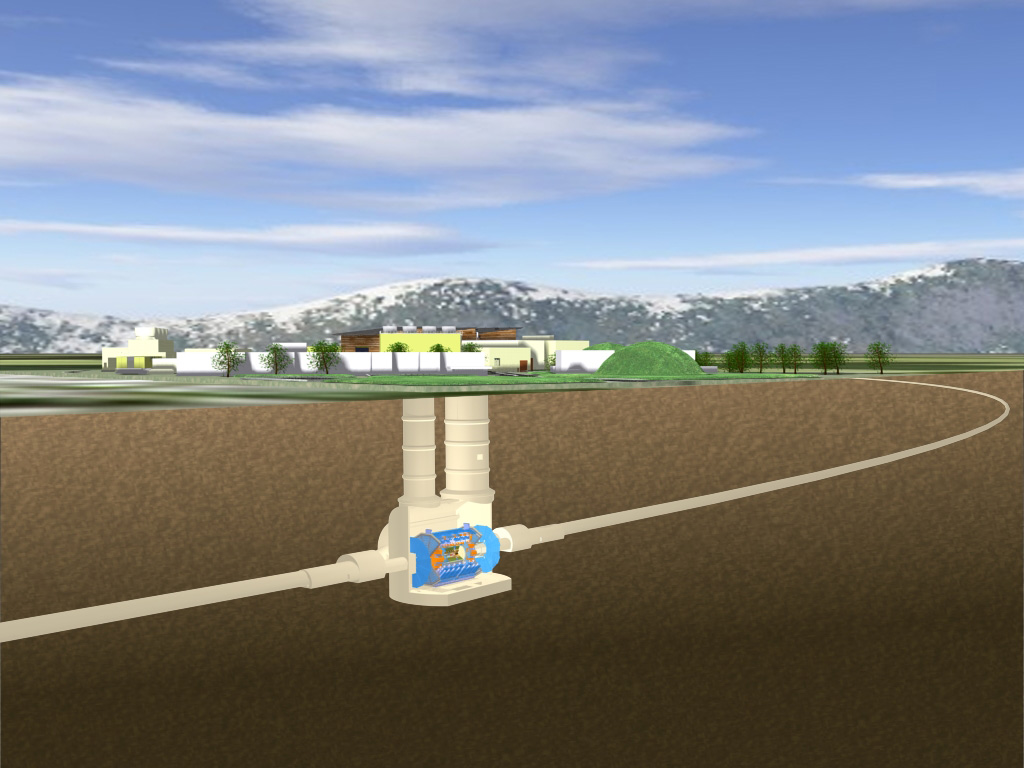
\includegraphics[width=0.8\textwidth]{dates/mtg/figures/atlas/ATLASUG}

}

% ATLAS experiment
\slide{ ATLAS experiment: details }
{
\centering
I mostly worked with Inner Detector (Pixel and SCT) and Muon Spectrometer. \\
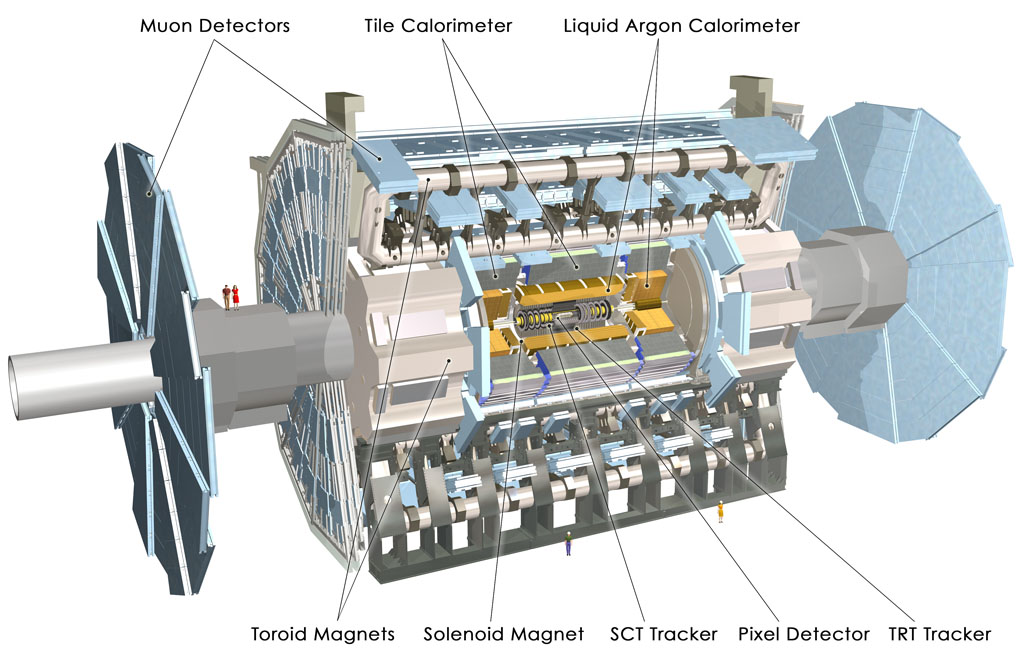
\includegraphics[width=0.8\textwidth]{dates/mtg/figures/atlas/ATLAS}

}

% ID zoom
\slide{ Inner Detector }
{
\colb[T]
\column{.5\textwidth}
\centering
Pixel and SCT trackers:
\iteb
\item Submerged in 2T solenoid B-field
\item Measure trajectories of charged particles w. $\mathcal{O}(11)$ tracking layers
\item Relatively small size (1 meter)
\item But highly-granular: \red{86M channels}
\iteb
\item \red{98\%} of ATLAS total!
\itee
\item Readout digitized \red{every 25 ns}
\itee

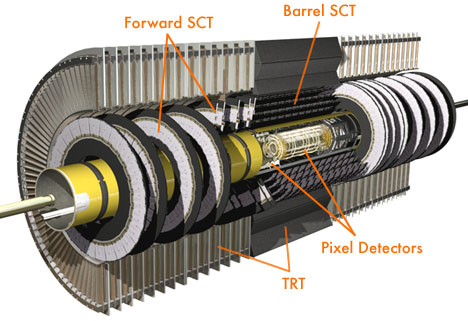
\includegraphics[width=1.0\textwidth]{dates/mtg/figures/atlas/ID2}

\column{.5\textwidth}

\centering
\tiny{A close-up view of silicon tracking layers:} \\
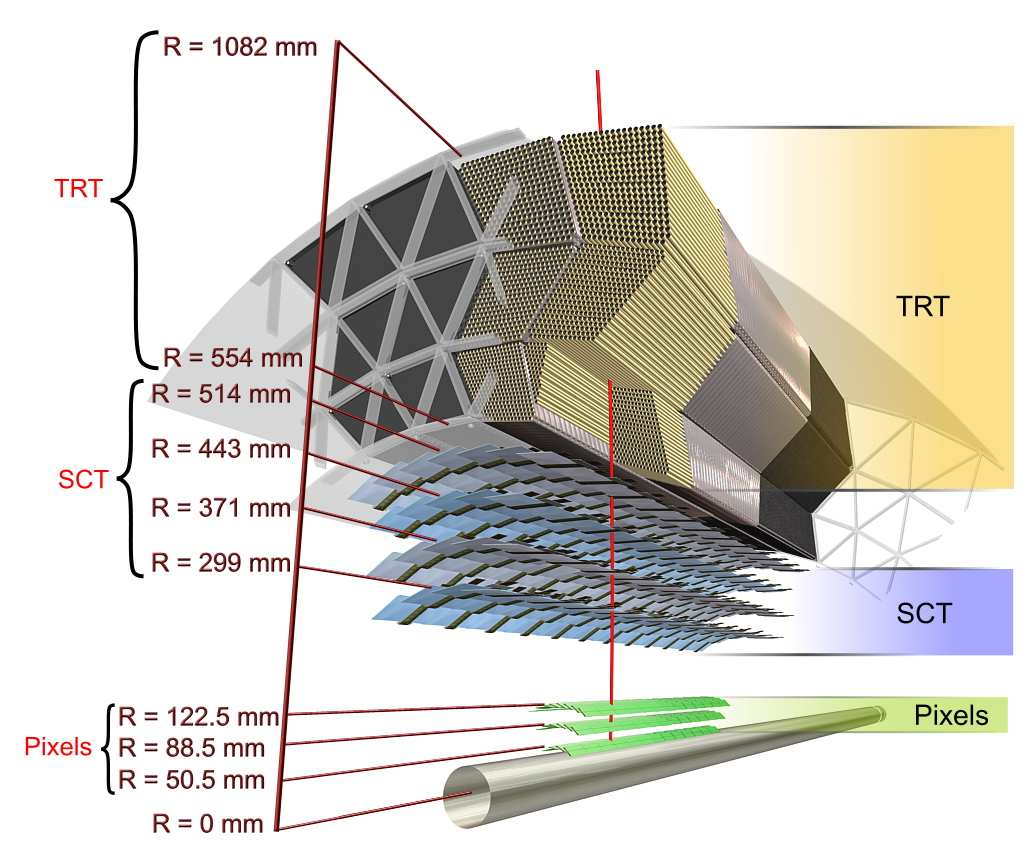
\includegraphics[width=1.0\textwidth]{dates/mtg/figures/atlas/ID}

\cole
}

% Trigger system
\slide{ Trigger system and FTK }
{
\centering
\iteb
\item 40 million events/sec. Each event $\mathcal{O}(1MB)$ $\rightarrow$ \red{1 Library of Congress/sec}
\item Can only save to disk $\mathcal{O}(200)$ events/sec $\rightarrow$ three-stage reduction system
\item Tracking would be a powerful tool to select interesting physics events
\iteb
\item Impossible combinatorial problem at LVL1; very hard (and limited) at LVL2
\itee
\item FTK: hardware system that reconstructs tracks with $pT>1 GeV$ at LVL1 rate
\itee

\colb[T]
\column{.4\textwidth}
\centering
\tiny{Example of track-based selection}:
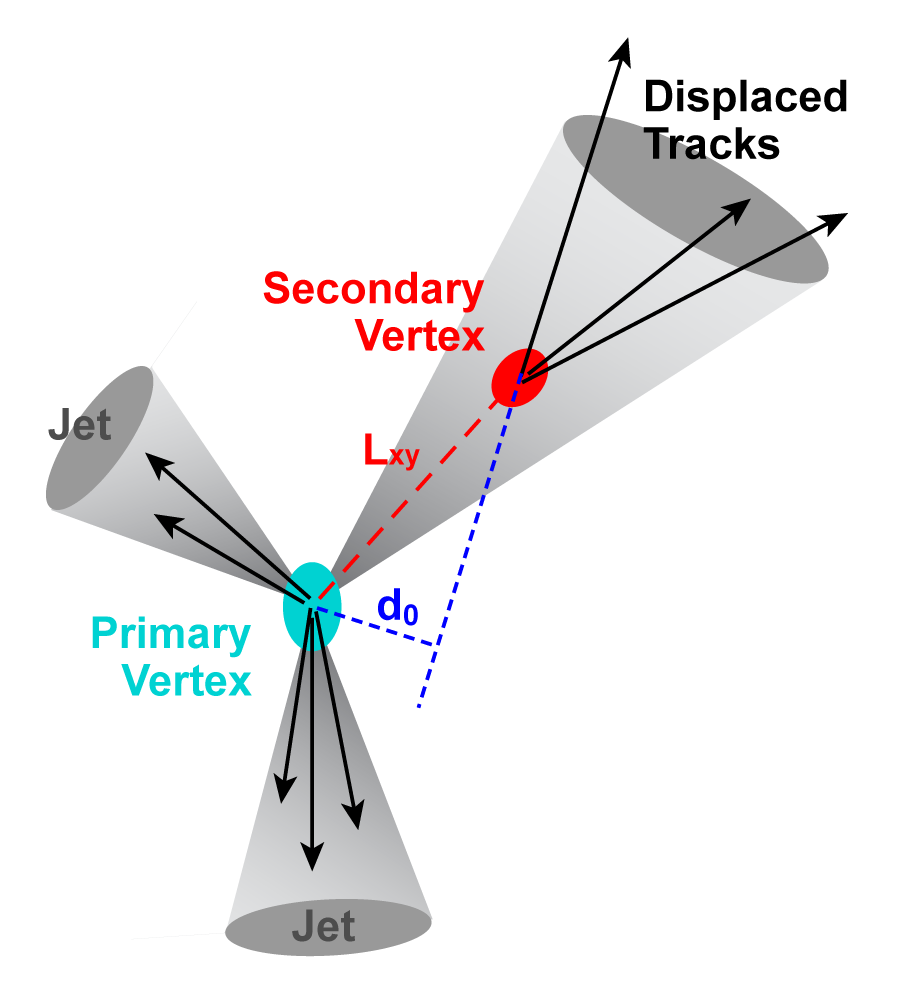
\includegraphics[width=.8\textwidth]{dates/mtg/figures/atlas/btag}
\column{.6\textwidth}
\centering
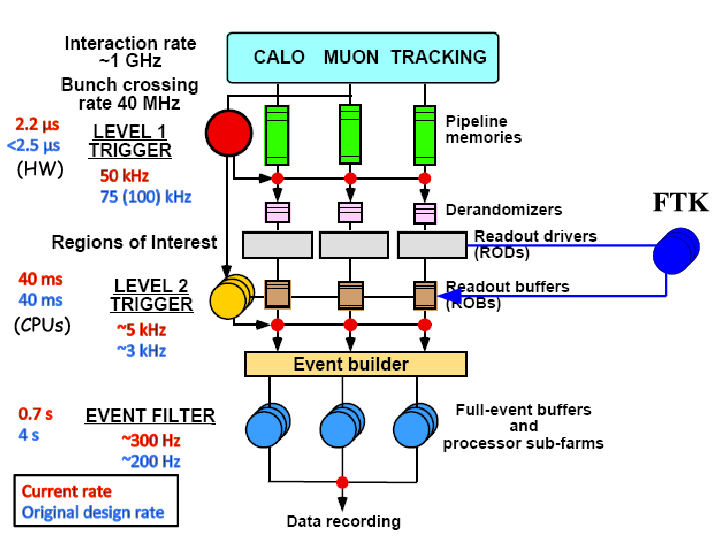
\includegraphics[width=1.0\textwidth]{dates/mtg/figures/atlas/trigger}
\cole

}

% FTK scheme
\slide{ FTK: principle of operation }
{
\centering
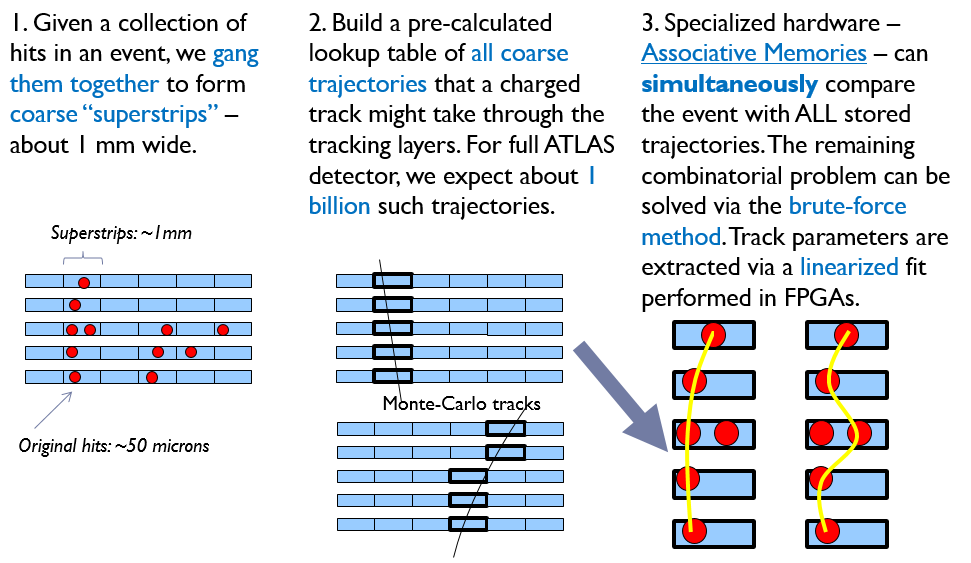
\includegraphics[width=1.0\textwidth]{dates/mtg/figures/atlas/ftk_principle} \\

All this takes just 30 $\mu$s per event - \red{x1000 faster than status quo}.

}

% FTK simulation
\slide{ 2006-2010: FTK software and simulations }
{
I wrote a lot of software to simulate FTK and evaluate its performance.
\iteb
\item Each event requires $\mathcal{O}(100)$ CPUs to simulate $\rightarrow$ use the Grid
\item Preparation of billions of coarse track trajectories is challenging
\item Unprecedented level of parallelism: $500k$ CPU-hours in 1 week
\itee

\centering
\tiny{ Example of FTK performance plot: impact parameter significance } \\
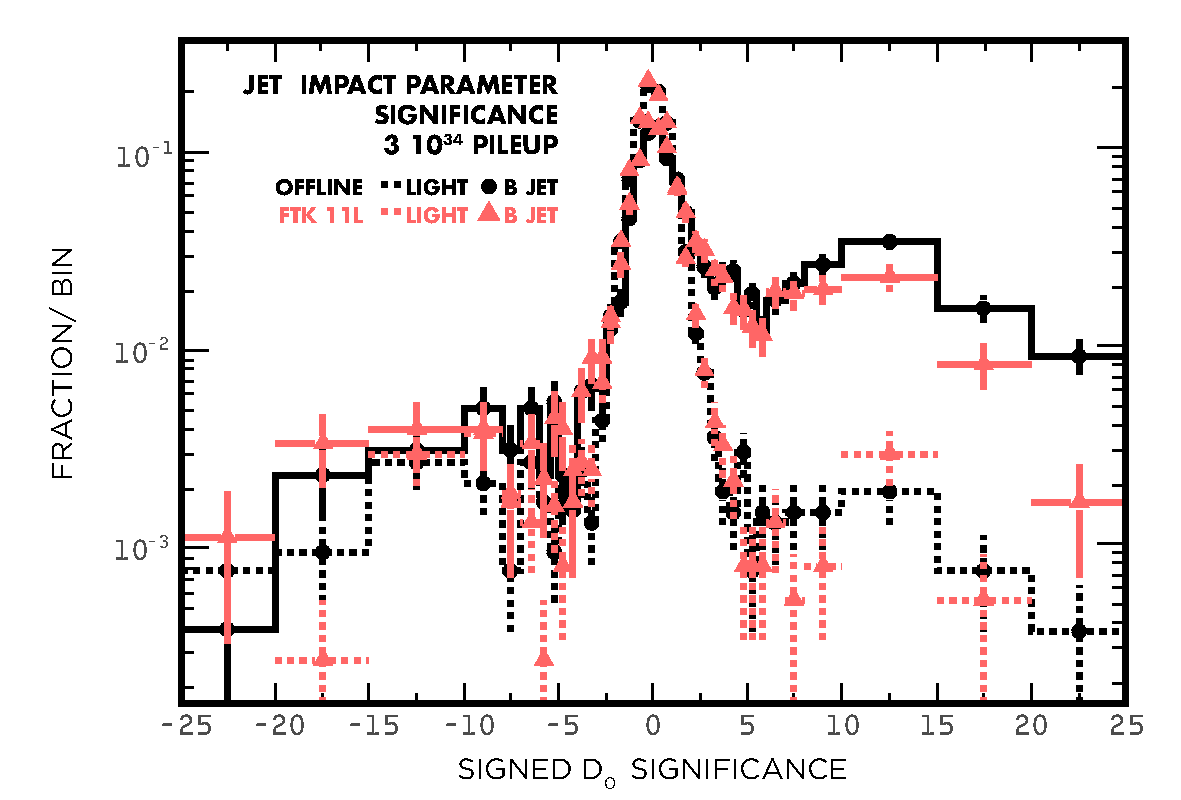
\includegraphics[width=0.6\textwidth]{dates/mtg/figures/atlas/d0sig}

}

% FTK hardware
\slide{ 2011-2012: FTK hardware }
{
FTK is currently in-development (TDR due this month). \\
But the \red{first piece of hardware is already finished}:
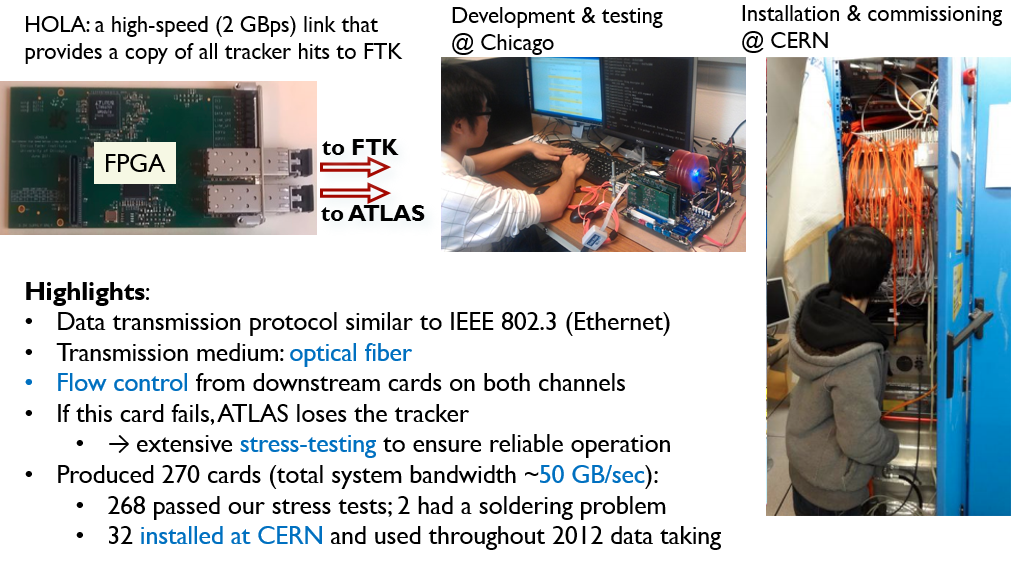
\includegraphics[width=1.0\textwidth]{dates/mtg/figures/atlas/hola}
}

% Trigger validation
\slide{ 2012-2013: ATLAS Trigger Validation }
{
\iteb
\item FTK is now part of the ATLAS Trigger group
\iteb
\item As such, we gained some operational responsibilities
\itee
\item Daily trigger validation:
\iteb
\item ATLAS trigger software consists of $\mathcal{O}(1000)$ packages
\item Dozens of developers regularly commit code and break things
\item Each day, a server farm runs unit tests to ensure all packages work
\itee
\item Chicago's Trigger Validation Framework:
\iteb
\item Automatically parses 1000's of logs to detect and classify errors
\item Maintains links to a bug tracker, which provides feedback to developers
\item Reduces shifter's time commitment from 6-8 hours to 1-2 hours per day.
\itee
\itee
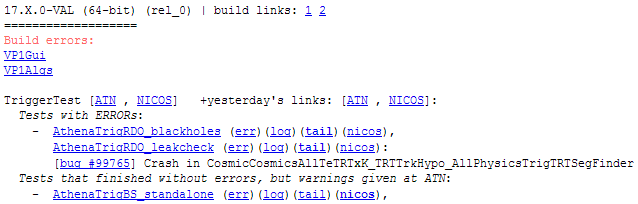
\includegraphics[width=0.8\textwidth]{dates/mtg/figures/atlas/shifts}
}

% ANALYSIS
\slide{ Analysis activities }
{
  Let's shift gears towards physics analysis activities.
}

% Muon momentum
\slide{ 2010-2011: muon momentum scale }
{
\colb[T]
\column{.5\textwidth}
\centering
\iteb
\item Muon momentum is not well-modeled in MC
\iteb
\item Imperfect detector alignment
\item Material distribution
\item Magnetic field
\itee
\item Z bosons as a standard candle
\iteb
\item ``Clean'' decay into two muons
\item Very small backgrounds
\item Fully reconstructible
\item Used to correct MC towards data
\itee
\item More details in the backup slides
\itee
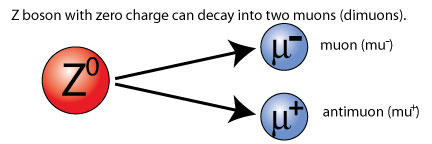
\includegraphics[width=0.8\textwidth]{dates/mtg/figures/mcp/z0decay} \\
\column{.5\textwidth}
\centering
\tiny{BEFORE: ATLAS default MC}\\
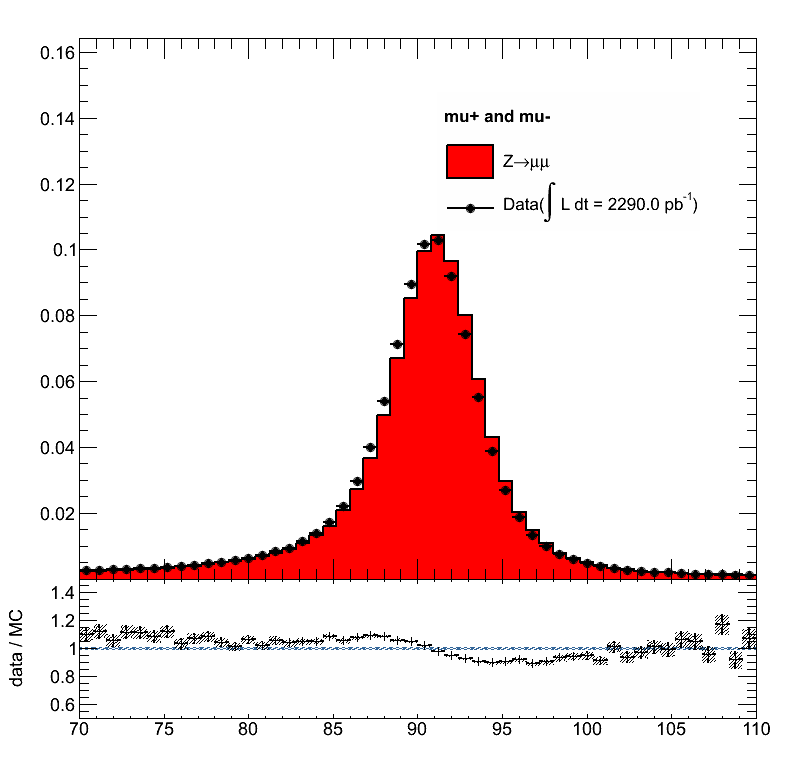
\includegraphics[width=0.65\textwidth]{dates/mtg/figures/mcp/KC_old} \\
\tiny{AFTER: utilizing our corrections}\\
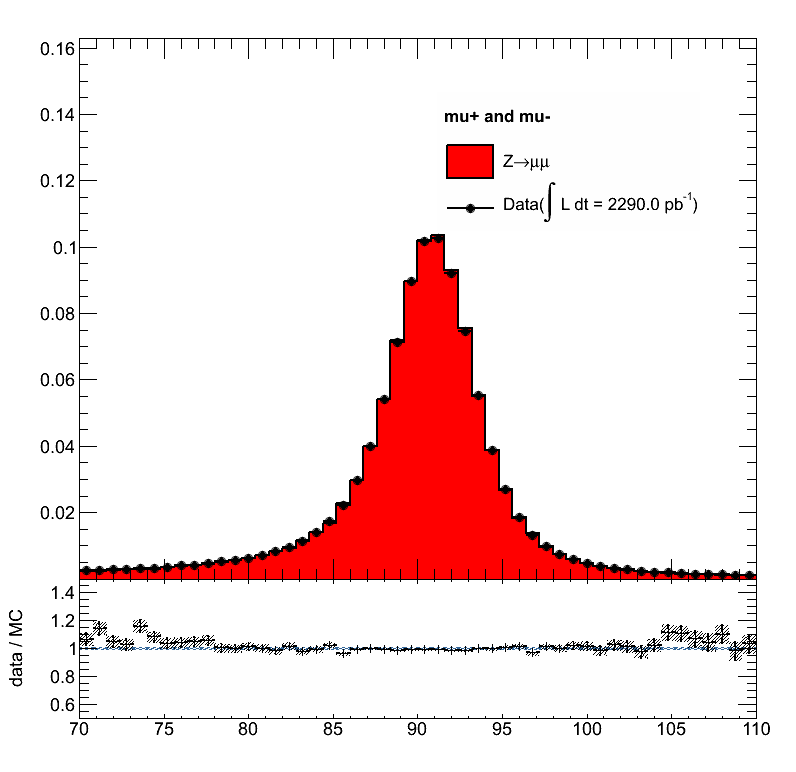
\includegraphics[width=0.65\textwidth]{dates/mtg/figures/mcp/KC_new}
\cole
 
}

% ANALYSIS
\slide{ Thesis topic }
{
  \begin{columns}
    \begin{column}{0.5\textwidth}
      \begin{tikzpicture}
        \begin{scope}
          [small mindmap,
          every node/.style={concept, execute at begin node=\hskip0pt, concept color=BrickRed, circular drop shadow, minimum size=1.8cm},
          every child/.style={concept color=BrickRed!100!gray!100, font=\large},
          concept/.append style={fill=BrickRed,text=white},
          grow cyclic,
          level 1/.append style={level distance=3.4cm, sibling angle=90}]
          \node [concept color=black, fill=white, text=black, minimum size=2.8cm] {7\,TeV \mbox{Inclusive W/Z} Cross~Section Measurement}[clockwise from=135]
          child [visible on=<1->] { node (Zee) {\Zee} }
          child [visible on=<1->] { node (Zmumu) {\Zmm} }
          child [visible on=<1->] { node (Wmunu) {\Wmn} }
          child [visible on=<1->] { node (Wenu) {\Wen} }
          ;
        \end{scope}
      \end{tikzpicture}

    \end{column}
    \begin{column}{0.5\textwidth}<1->
      \begin{itemize}
      \item \textit{``Measurement of differential inclusive W boson production and decay cross sections in the muon channel using the ATLAS Detector.''}
      \item Part of the comprehensive W/Z cross-section measurement paper at ATLAS
      \end{itemize}
    \end{column}
  \end{columns}

}

% measurement details
\slide{Measurement details}
{
  Highlighted in \red{red} are my contributions:
  \vspace{-.1cm}
  \begin{itemize}
  \item Integrated \red{W} and Z \red{cross-sections and ratios}, statement on $W\to
    e\nu/W\to\mu\nu$ for Lepton universality constraint
  \item \red{$W^+$, $W^-$ lepton pseudorapidity $\eta_\ell$ differential}
  \item $Z/\gamma^*$ boson rapidity differential in $y_{\ell\ell}$ (central and forward Z) in
    three coarse mass bins on and off the Z peak $m_{\ell\ell} = 46 -
    66 - 116 - 150$ GeV (difference in scale and $Z$ and $\gamma^*$ couplings)
  \item \red{$W^+$, $W^-$ lepton $\eta_\ell \times p_{T,\ell}$
    differential}: understanding lepton $p_T$ (cut)
    modelling in MC and fixed order programs
  \item A finer 1D mass-binned cross-section in $m_{\ell\ell} =
    66-76-91-106-116$ GeV for combination with low + high mass DY
    analyses in one plot
  \item NNLO QCD fit to test data compatibility and impact; test large
    strange content of the proton found with 2010 data
  \end{itemize}
  \vspace{.3cm}
  \begin{itemize}
  \item Critically depends on \red{understanding of lepton and $\met$
    performance} as well as precise luminosity measurements
  \item Large improvement in precision w.r.t. the 2010 publication
  \item \blue{Current status: } measurements are largely finished. A 550-page internal note written. ATLAS approval in-progress.
  \end{itemize}

}

% SM
\slide{ Standard Model }
{
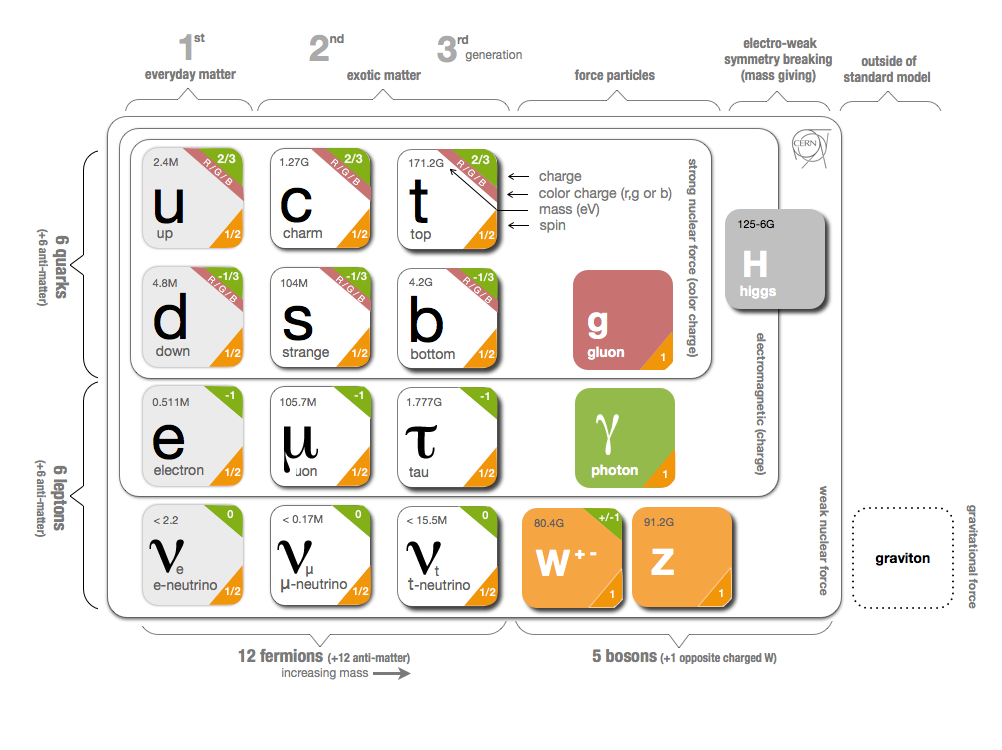
\includegraphics[width=0.9\textwidth]{dates/mtg/figures/wz/sm}
}

\slide{ W boson: production }
{
\colb[T]
\column{.6\textwidth}
\centering
\iteb
\item Protons can be viewed as collections of \red{partons}
\iteb
\item Valence quarks: Up+Up+Down
\item Sea quarks
\item Gluons
\itee
\item W bosons produced when two partons interact
\item Each parton carries a fraction of proton's energy
\iteb
\item These are measured empirically
\item Parton Distribution Functions (PDFs)
\itee
\item Production vertex: \red{perturbative} QCD
\iteb
\item Higher precision $\rightarrow$ beyond leading order
\item NLO: 3\% from reno./fact. scale variations
\item NNLO: $<1\%$ from reno./fact. scale
\itee
\itee
\column{.4\textwidth}
\centering
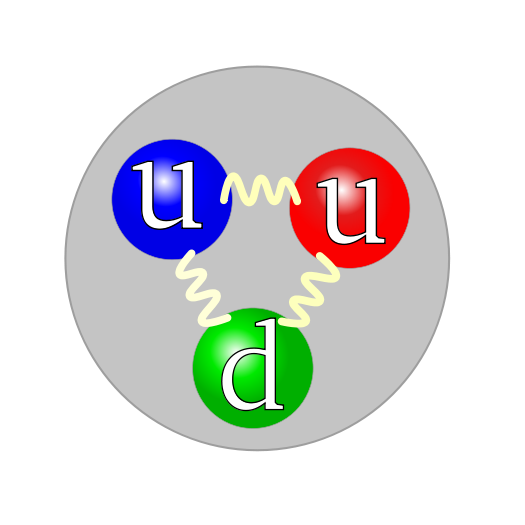
\includegraphics[width=0.3\textwidth]{dates/mtg/figures/wz/proton} \\
\tiny{ Process at leading order (LO): } \\
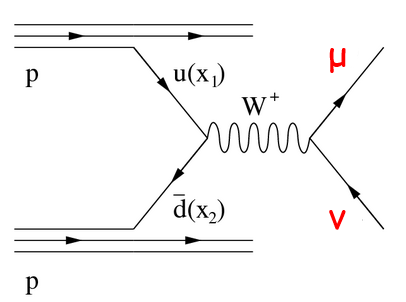
\includegraphics[width=0.6\textwidth]{dates/mtg/figures/wz/wmunuf} \\
\tiny{ Process at next-to-leading order (NLO): } \\
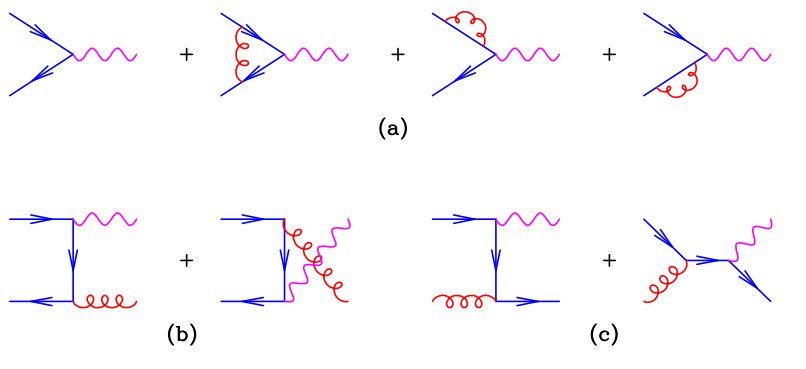
\includegraphics[width=1.0\textwidth]{dates/mtg/figures/wz/nlo} \\
\cole
}

\slide{ W boson: why it's interesting }
{
\colb[T]
\column{.6\textwidth}
\centering
\iteb
\item Proton structure
\iteb
\item Validate existing PDF predictions
\item Provide new constraints for future expt's
\item E.g., cross-section vs $\eta$ (see figure)
\itee
\item Tests of perturbative QCD
\iteb
\item Last published measurement: 2010 data
\item Achieved precision: $\mathcal{O}(2-3\%)$
\item Today, we can finally reach below 1\%
\itee
\item Better understanding of the detector
\iteb
\item People focus on Higgs, new physics
\item These analyses don't need percent-level understanding of the detector
\item We can fill the gap
\itee
\itee
\column{.4\textwidth}
\centering
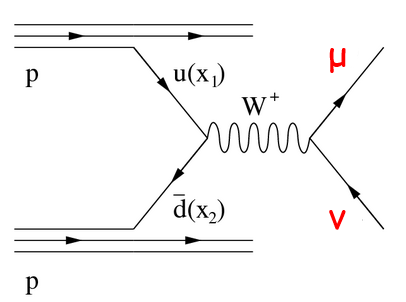
\includegraphics[width=0.6\textwidth]{dates/mtg/figures/wz/wmunuf} \\
\tiny{ Explaining pseudorapidity ($\eta$): } \\
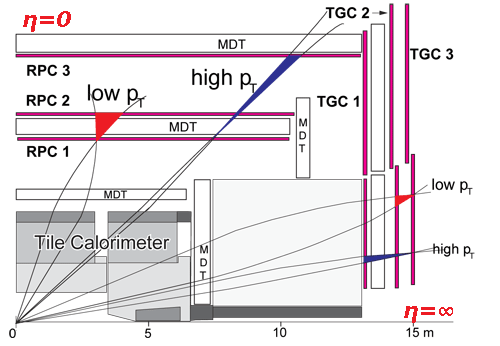
\includegraphics[width=1.0\textwidth]{dates/mtg/figures/wz/eta} \\
\cole
}

\slide{ W boson: decay via $W \rightarrow \mu \nu$ }
{
\centering
\iteb
\item Muons are measured from tracker hits and muon spectrometer stations
\item Neutrinos escape undetected - but we measure ``missing energy''
\itee
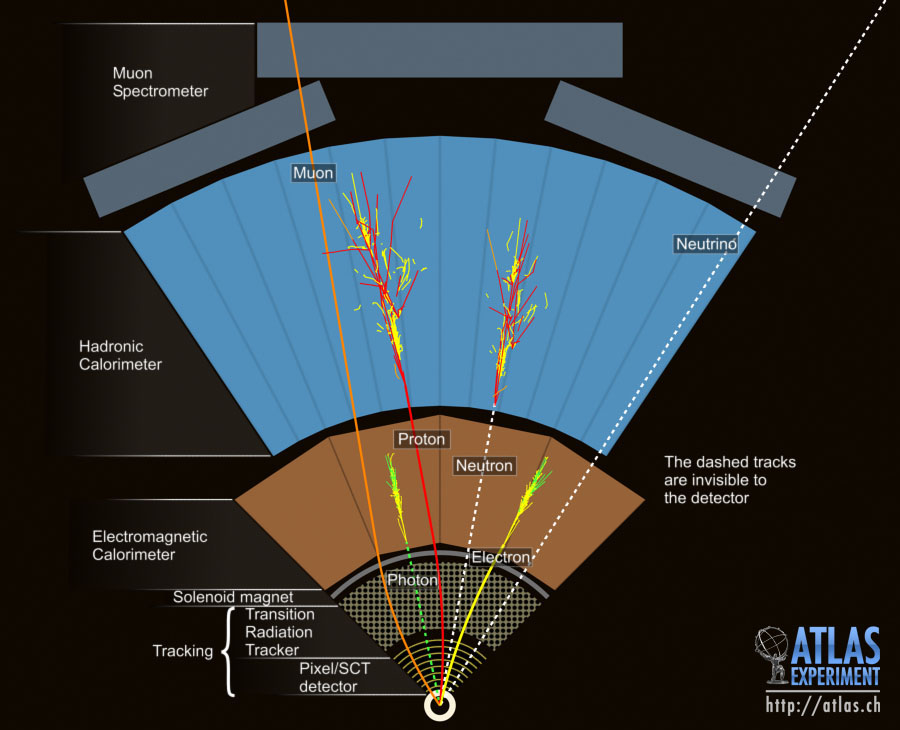
\includegraphics[width=0.7\textwidth]{dates/mtg/figures/wz/particles}

}

%% /home/antonk/SupportingDocument/


% why 2011 - pt.1
\begin{frame}{It's 2013. Why still use 2011 data?}
\begin{itemize}
\item All 2011 analyses used a trigger recommended by muon experts
\item We discovered disagreements in left-vs-right side of the detector
\end{itemize}

\centering
\includegraphics[width=0.4\textwidth]{/home/antonk/SupportingDocument/Wmunu/figures/AC/old/W_NOM_Q0_stack_d3_eta_lpt_met_y_2__1_z_0__1_NEG}
\includegraphics[width=0.4\textwidth]{/home/antonk/SupportingDocument/Wmunu/figures/AC/old/W_NOM_Q0_stack_d3_eta_lpt_met_y_2__1_z_0__1_POS}

~~~~~~~~~~~~~~~~~~~~~~~~~~~~~~~~~~~~~~$W^-$~~~~~~~~~~~~~~~~~~~~~~~~~~~~$W^+$
\end{frame}

% why 2011 - pt.2
\begin{frame}{It's 2013. Why still use 2011 data?}
\begin{itemize}
\item After the trigger problem was understood, we proposed a solution
\item Left-vs-right side agree within uncertainties
\end{itemize}

\centering
\includegraphics[width=0.4\textwidth]{/home/antonk/SupportingDocument/Wmunu/figures/AC/new/W_NOM_Q0_stack_d3_eta_lpt_met_y_2__1_z_0__1_NEG}
\includegraphics[width=0.4\textwidth]{/home/antonk/SupportingDocument/Wmunu/figures/AC/new/W_NOM_Q0_stack_d3_eta_lpt_met_y_2__1_z_0__1_POS}

~~~~~~~~~~~~~~~~~~~~~~~~~~~~~~~~~~~~~~$W^-$~~~~~~~~~~~~~~~~~~~~~~~~~~~~$W^+$
\end{frame}


%  Selection
\slide{W,Z selection in muon channels}
{
Common selection:
\iteb
\item \textit{Single muon triggers}: EF\_mu18 or EF\_mu18\_medium
\item Primary vertex with $\ge$ 3 tracks
\item Reject events with $BadLooser$ jets or jets in $LarHole$ region
\item Combined STACO muons passing MCP quality cuts and $|z_0|~<~10~mm$
\item Muon kinematics: $p_T~>~25~\GeV$ and $|\eta|~<~2.4$
\item Tracking isolation: $\sum \pt(\Delta R~<~0.4) / \pt~<~0.1$
\itee
\textbf{\large $\mathbf{W \to \mu\nu}$ channel}:
\iteb
\item \textit{Exactly one isolated muon}
\item $\met > 25\,\GeV$, $\mt > 40\,\GeV$ using \texttt{MET\_RefFinal}
\itee
\textbf{\large $\mathbf{Z \to \mu\mu}$ channel}:
\iteb
\item \textit{Exactly two isolated muons}
\item Opposite charges
\item $46 < m_{\mu\mu} < 150\gev$
\itee
}

% background
\slide{Backgrounds}
{
\iteb
\item Small backgrounds from other \Zll\ and \Wln\ channels, Dibosons,
  $t\bar{t}$ and single $t$ are estimated from MCs
\iteb
\item $\Zmm$ and $\Wmn$: Powheg+Pythia, Powheg+Herwig, MCNLO
\item $\tau$ samples: Alpgen+Jimmy, rapidity-reweighted
\item dibosons: Herwig
\item top: MCNLO
\itee
\item Main work is multijet background estimation to permil level
\iteb
\item Short summary on the next slide
\itee
\itee
}

% qcd
\slide{Multi-jet background in \Wmn}
{
\colb[t]
\column{.6\textwidth}
\centering
\iteb
\item LHC produces a lot of jets
\item Heavy-flavor jets contain muons
\item Easy to mistake these for a W decay
\item Multi-jets are difficult to model in MC
\iteb
\item Data-driven fit in a control region
\item Non-isolated muons, $low-\met$ region
\itee
\itee
\includegraphics[width=0.65\textwidth]{/home/antonk/SupportingDocument/Wmunu/figures/qcdfits/Q0_x_1_1_y_1_1}

\column{.4\textwidth}
\centering
\small{Multi-jet fraction and error:} \\
\includegraphics[width=0.70\textwidth]{/home/antonk/SupportingDocument/Wmunu/figures/qcdunc/Q1_qcd_ptALL25_etaLOOP_ewk_frac} \\
\includegraphics[width=0.70\textwidth]{/home/antonk/SupportingDocument/Wmunu/figures/qcdunc/Q0_qcd_ptALL25_etaLOOP_ewk_frac}

\cole
}

% stacks
\slide{Control plots} 
{
\only<1>{$\Wminus  \rightarrow \mu^-\nu$}
\only<2>{$\Wplus  \rightarrow \mu^{+} \nu$}
\scriptsize{(Systematic band includes all experimental uncertainties + MC generators + boson $p_{T}$.)}

\vspace{-.3cm}
 \begin{columns}
  \begin{column}{0.32\textwidth}
     \begin{center}
       Muon $\eta$ \\
       \vspace{-.03cm}
       \includegraphics[width=1.00\textwidth]<1>{/home/antonk/SupportingDocument/Wmunu/figures/control_plots/inclusive25/P_stack_d3_eta_lpt_met_y_2__1_z_0__1_NEG}
       \includegraphics[width=1.00\textwidth]<2>{/home/antonk/SupportingDocument/Wmunu/figures/control_plots/inclusive25/P_stack_d3_eta_lpt_met_y_2__1_z_0__1_POS}
     \end{center}
     \vspace{-.7cm}
     \begin{center}
       Muon $p_T$ \\
       \vspace{-.03cm}
       \includegraphics[width=1.00\textwidth]<1>{/home/antonk/SupportingDocument/Wmunu/figures/control_plots/inclusive25/P_stack_lpt_NEG}
       \includegraphics[width=1.00\textwidth]<2>{/home/antonk/SupportingDocument/Wmunu/figures/control_plots/inclusive25/P_stack_lpt_POS}
     \end{center}
  \end{column}

  \begin{column}{0.32\textwidth}
     \begin{center}
       $E_T^{Miss}$ \\
       \vspace{-.03cm}
       \includegraphics[width=1.00\textwidth]<1>{/home/antonk/SupportingDocument/Wmunu/figures/control_plots/inclusive25/P_stack_d3_abseta_lpt_met_x_0__1_y_2__1_NEG}
       \includegraphics[width=1.00\textwidth]<2>{/home/antonk/SupportingDocument/Wmunu/figures/control_plots/inclusive25/P_stack_d3_abseta_lpt_met_x_0__1_y_2__1_POS}
     \end{center}
     \vspace{-.7cm}
     \begin{center}
       $m_T^{W}$ \\
       \vspace{-.03cm}
       \includegraphics[width=1.00\textwidth]<1>{/home/antonk/SupportingDocument/Wmunu/figures/control_plots/inclusive25/P_stack_d3_abseta_lpt_wmt_x_0__1_y_2__1_NEG}
       \includegraphics[width=1.00\textwidth]<2>{/home/antonk/SupportingDocument/Wmunu/figures/control_plots/inclusive25/P_stack_d3_abseta_lpt_wmt_x_0__1_y_2__1_POS}
     \end{center}
  \end{column}

  \begin{column}{0.32\textwidth}
     \begin{center}
       $p^{W}_{T}$ \\
       \vspace{-.03cm}
       \includegraphics[width=1.0\textwidth]<1>{/home/antonk/SupportingDocument/Wmunu/figures/control_plots/inclusive25/P_stack_d3_abseta_lpt_wpt_x_0__1_y_2__1_NEG}
       \includegraphics[width=1.0\textwidth]<2>{/home/antonk/SupportingDocument/Wmunu/figures/control_plots/inclusive25/P_stack_d3_abseta_lpt_wpt_x_0__1_y_2__1_POS}
     \end{center}
     \vspace{-.7cm}
     \begin{center}
       $Muon~\phi$ \\
       \vspace{-.03cm}
       \includegraphics[width=1.0\textwidth]<1>{/home/antonk/SupportingDocument/Wmunu/figures/control_plots/inclusive25/P_stack_d3_abseta_lpt_phi_x_0__1_y_2__1_NEG}
       \includegraphics[width=1.0\textwidth]<2>{/home/antonk/SupportingDocument/Wmunu/figures/control_plots/inclusive25/P_stack_d3_abseta_lpt_phi_x_0__1_y_2__1_POS}
     \end{center}
  \end{column}

\end{columns}
}

% summary of uncertainties
\slide{Summary of uncertainties for \Wmn}
{

Representative uncertainties for \red{$W^-$}: $p_{T}>25$, $25<p_{T}<30$, $40<p_{T}<45$
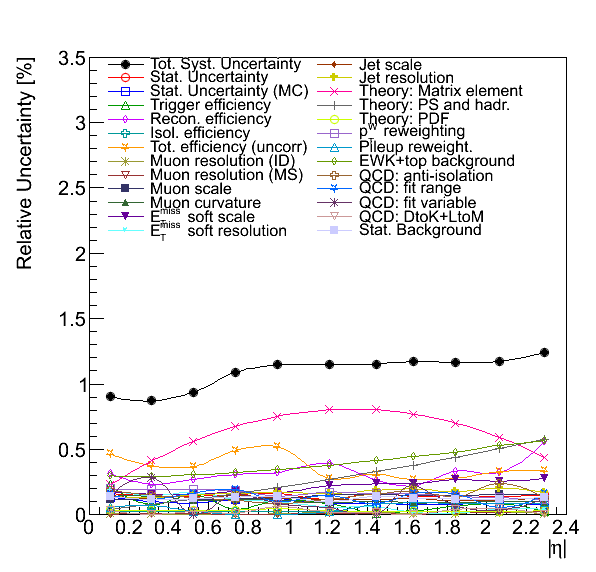
\includegraphics[width=0.32\textwidth]{/home/antonk/SupportingDocument/Wmunu/figures/res/Wmn_SYSTEM_1D_PT25_NEG_Unc_proj}
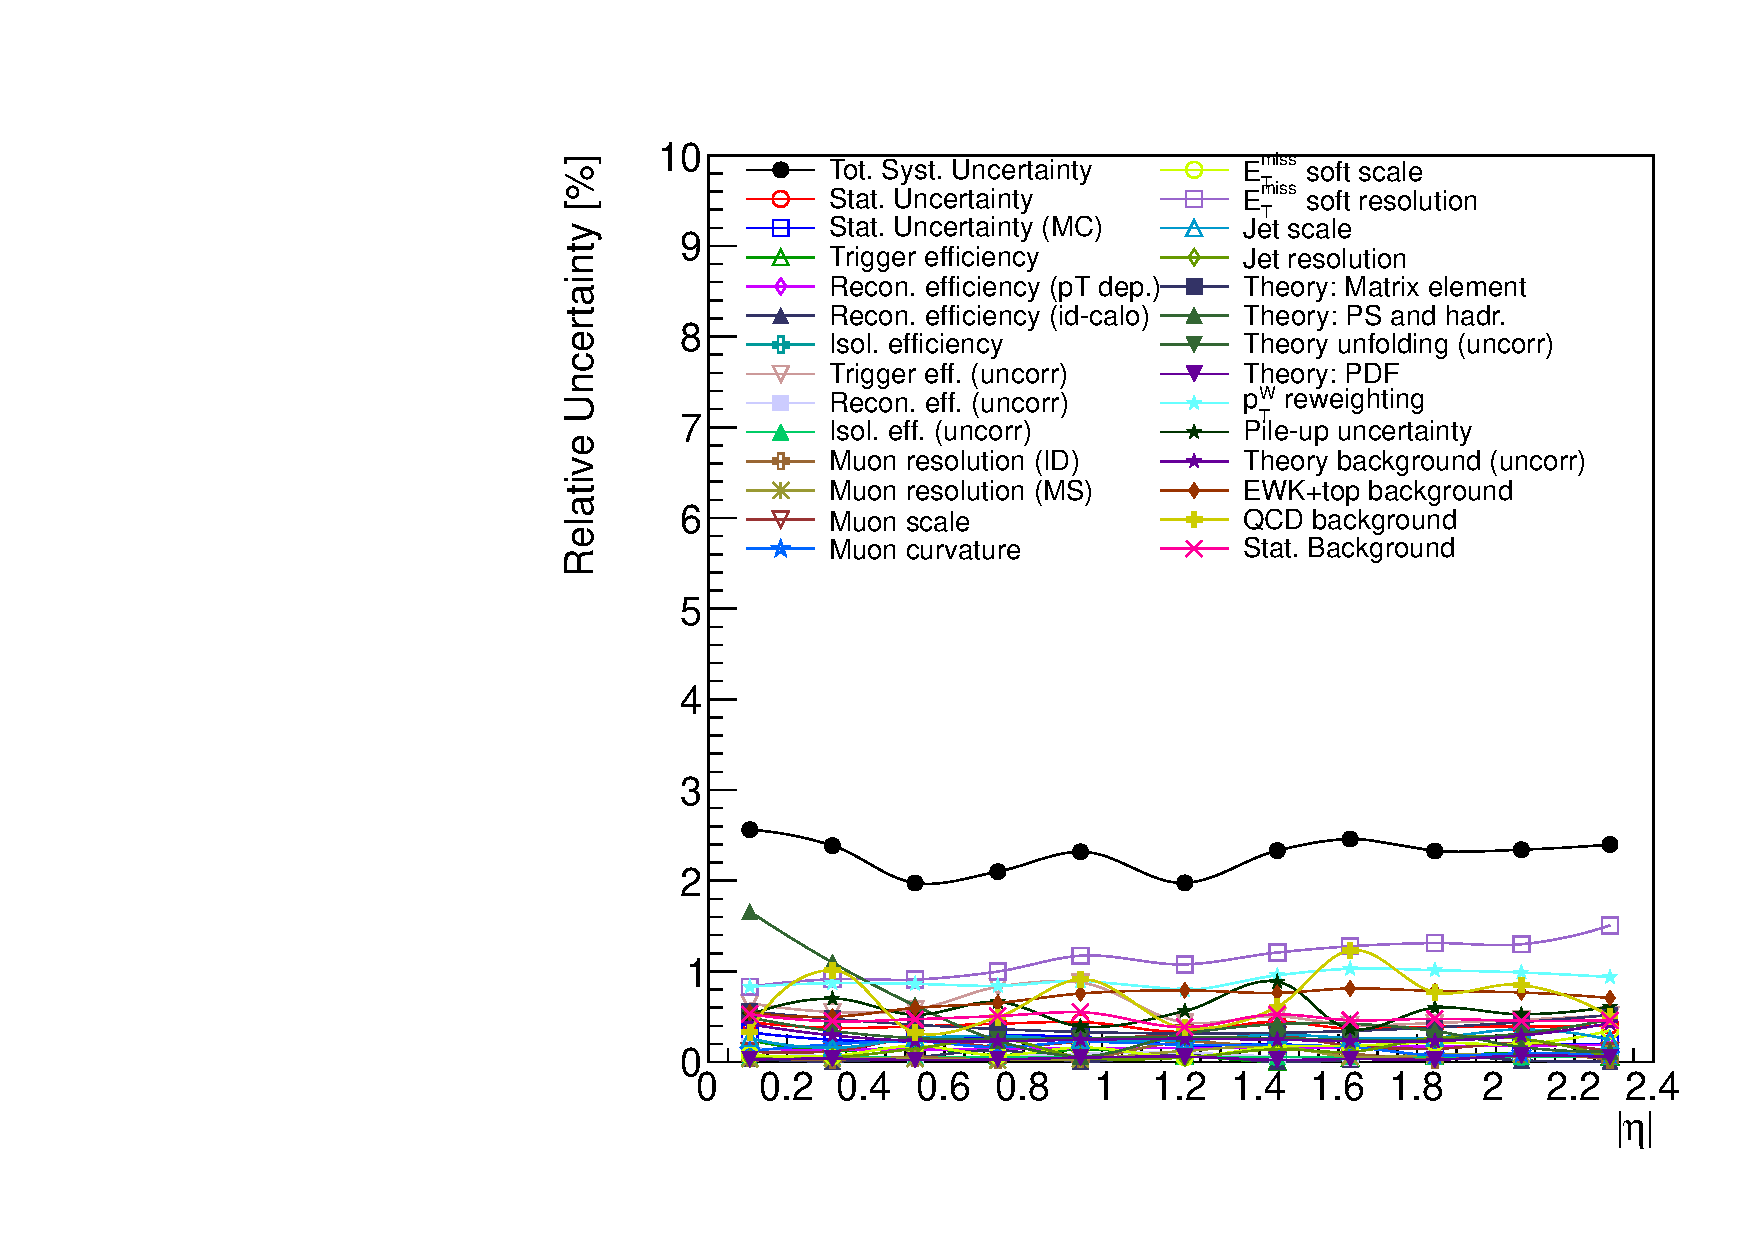
\includegraphics[width=0.32\textwidth]{/home/antonk/SupportingDocument/Wmunu/figures/res/Wmn_SYSTEM_2D_PT20_NEG_Unc_2d_Slice_2}
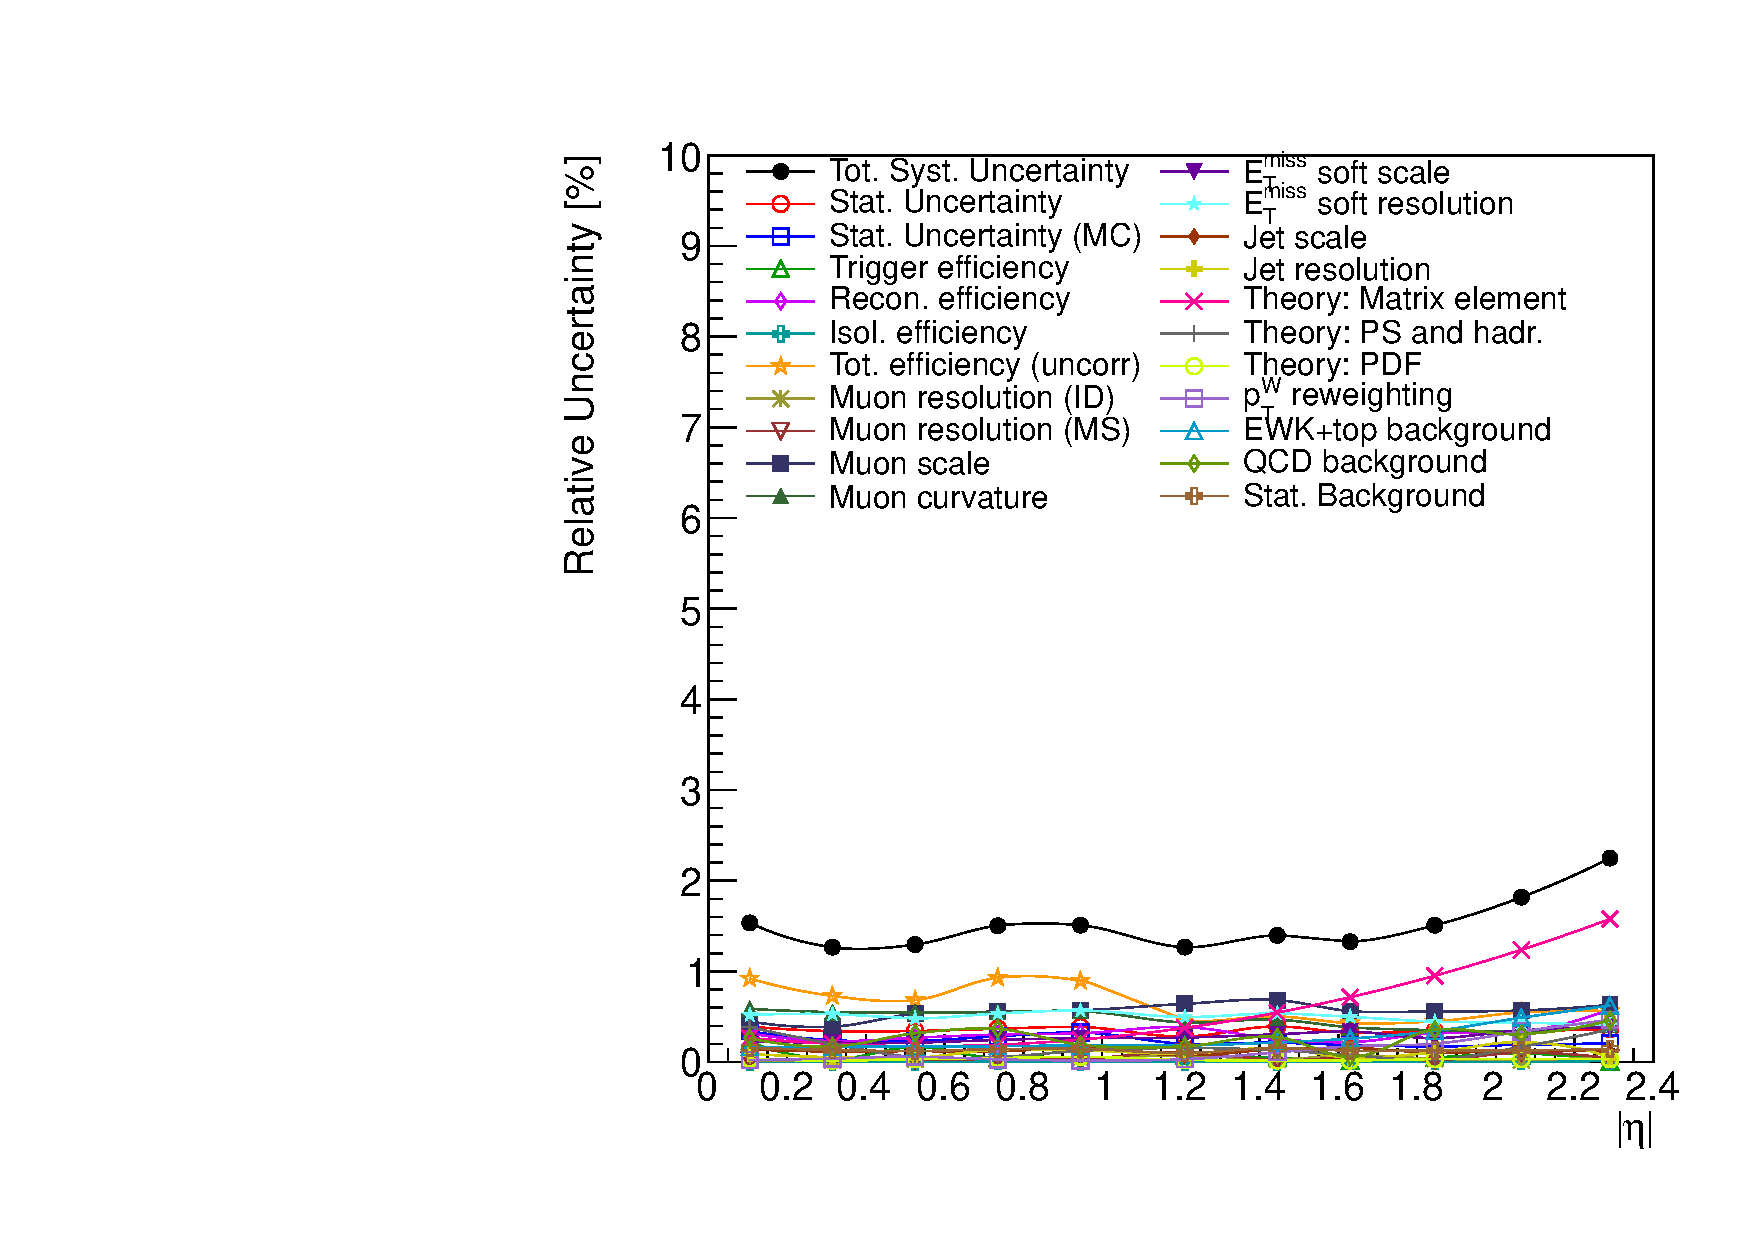
\includegraphics[width=0.32\textwidth]{/home/antonk/SupportingDocument/Wmunu/figures/res/Wmn_SYSTEM_2D_PT20_NEG_Unc_2d_Slice_5}

Representative uncertainties for \red{$W^+$}: $p_{T}>25$, $25<p_{T}<30$, $40<p_{T}<45$
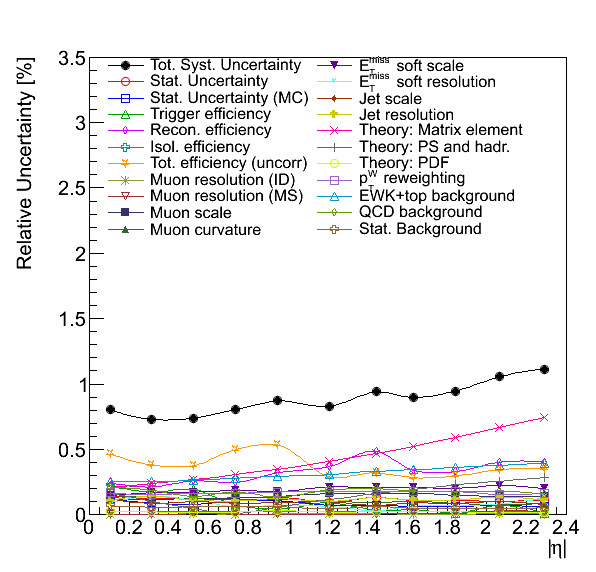
\includegraphics[width=0.32\textwidth]{/home/antonk/SupportingDocument/Wmunu/figures/res/Wmn_SYSTEM_1D_PT25_POS_Unc_proj}
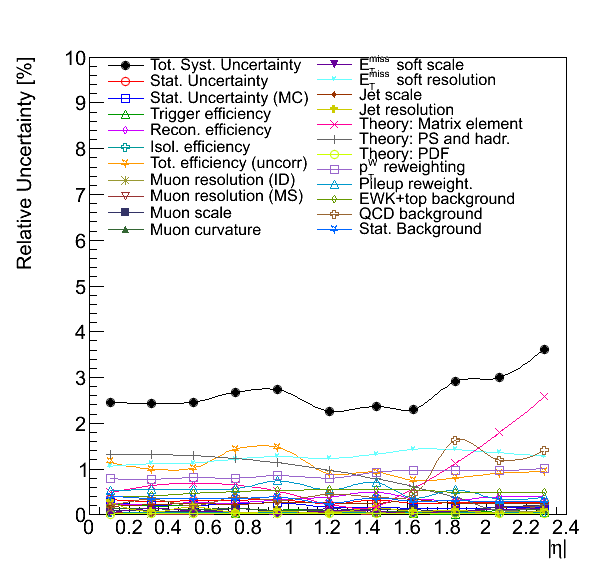
\includegraphics[width=0.32\textwidth]{/home/antonk/SupportingDocument/Wmunu/figures/res/Wmn_SYSTEM_2D_PT20_POS_Unc_2d_Slice_2}
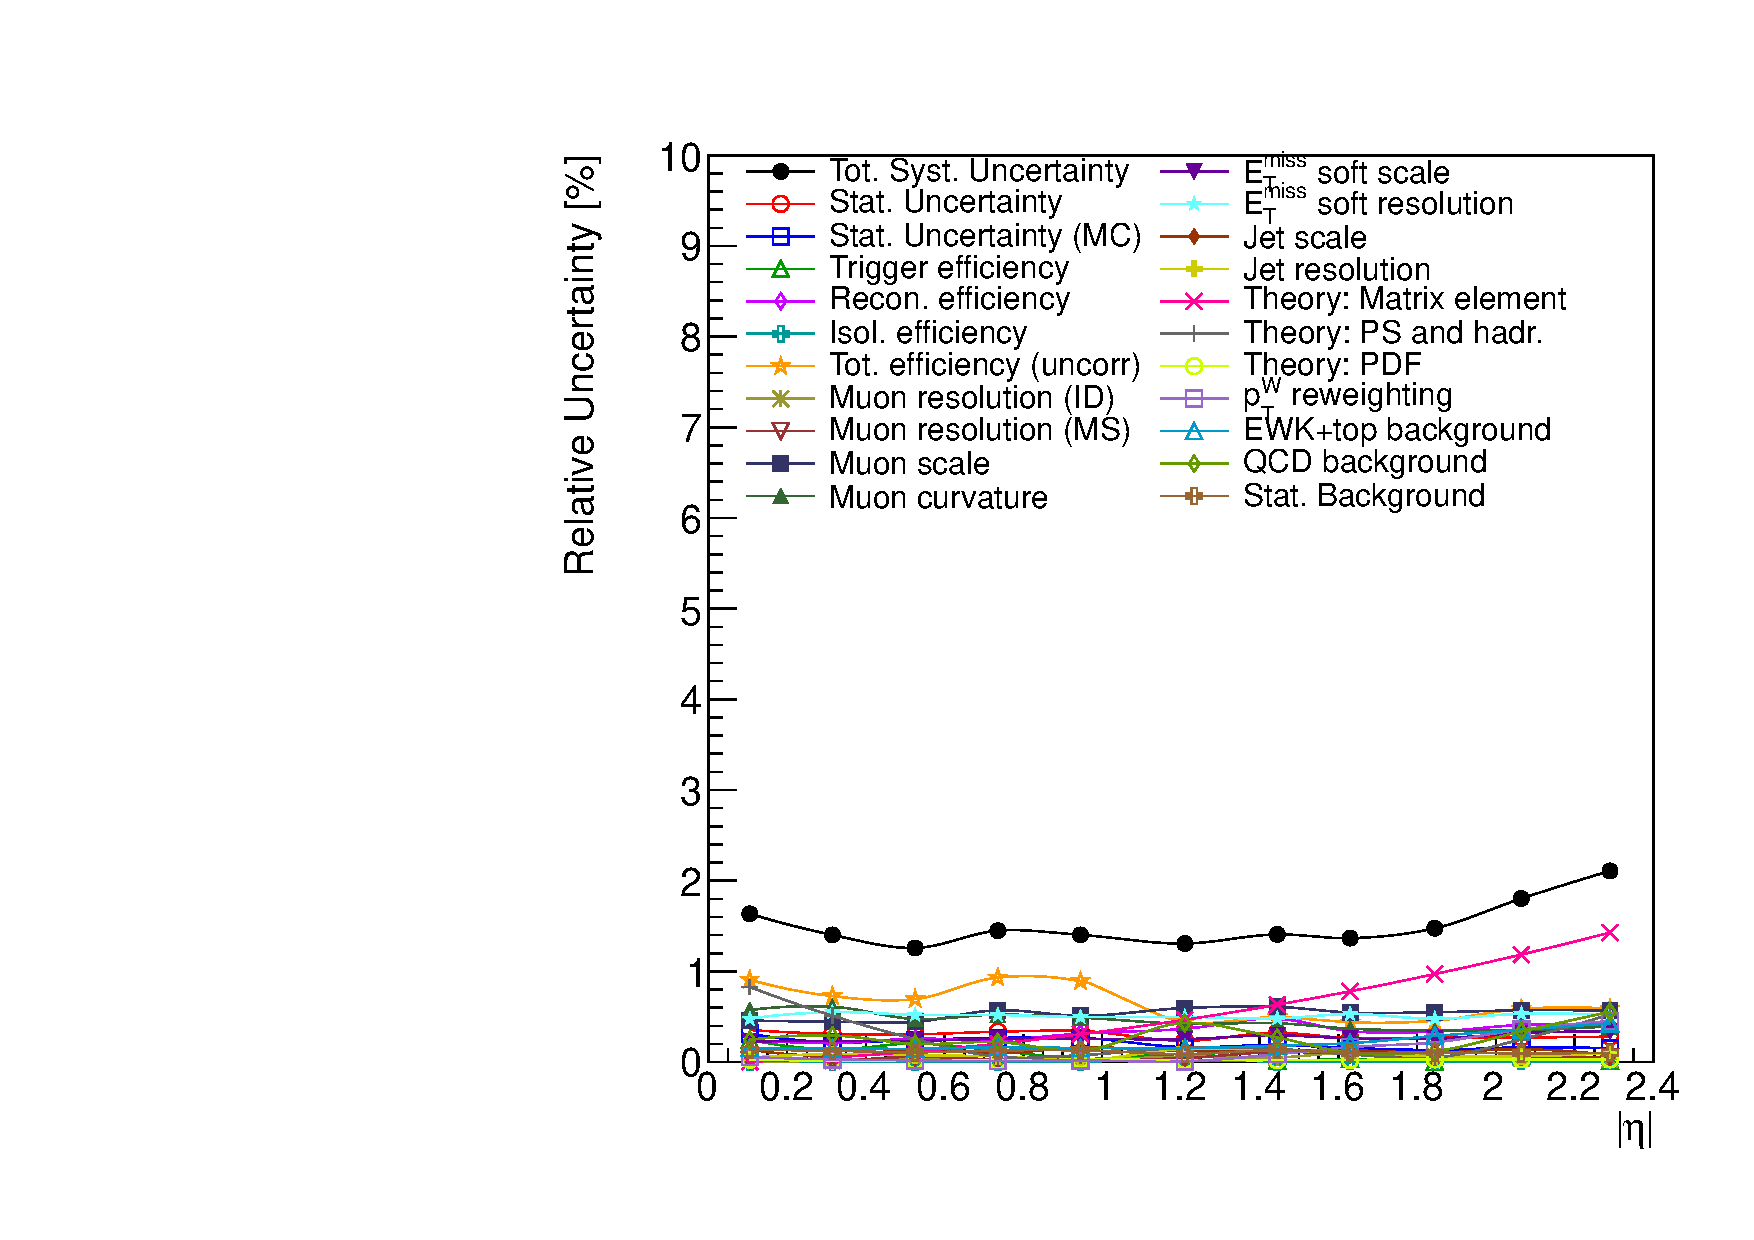
\includegraphics[width=0.32\textwidth]{/home/antonk/SupportingDocument/Wmunu/figures/res/Wmn_SYSTEM_2D_PT20_POS_Unc_2d_Slice_5}

}

% correlation between systematics
\begin{frame}{Correlation of Systematics}
  \tiny
  \centering
    \begin{tabular}{lccccc}
      \hline
      \hline
      & \multicolumn{5}{c}{Channel} \\
      Uncertainty Source & \Wen\ & \Zee\ & \Zee\ (CF) & \Wmn\ & \Zmm\  \\
      \hline
      \input{/home/antonk/SupportingDocument/tables/systematic_correlations.tex}
      \hline
      \hline
    \end{tabular}\\

    \normalsize
    \begin{itemize}
    \item $i$: Correlated between bins and channels
    \item u$i$: Uncorrelated between bins but correlated between channels
    \end{itemize}
\end{frame}

% combination
\begin{frame}{Comparison of $W^+$ (left) and $W^-$ cross-sections.}

 \centering
\begin{itemize}
\item \Wmn\ and \Wen\ measurements combined taking into account all correlations
\end{itemize}

   \includegraphics[width=0.45\textwidth]{/home/antonk/SupportingDocument/figures/WPeta25_ratio_combined}
   \includegraphics[width=0.45\textwidth]{/home/antonk/SupportingDocument/figures/WMeta25_ratio_combined}

\begin{itemize}
\item Overall combination $\chi^2/\mathrm{n.d.f} = 66.3/53$ (inc. $W^\pm$ and $Z/\gamma^*$)
\end{itemize}

\end{frame}

% nnlo plots
\begin{frame}{NNLO QCD + NLO EWK predictions, W channel}
\begin{itemize}
\item Theory error bars include uncertainty of PDF and $\alpha_S$
\item Power to constrain PDFs: MSTW disagreements at few-percent level
\item Predictions for other PDFs are under way
\end{itemize}
 \centering
  \includegraphics[width=0.45\textwidth]{/home/antonk/SupportingDocument/figures/WPeta25_NNLO_combined.pdf}
  \includegraphics[width=0.45\textwidth]{/home/antonk/SupportingDocument/figures/WMeta25_NNLO_combined.pdf}

left: $W^+$, right: $W^-$

\end{frame}

% PDF fits

\begin{frame}{Sensitivity study of W,Z 2011 data}

\begin{center}
\begin{columns}
\begin{column}{5cm}
 \includegraphics[width=\textwidth]{/home/antonk/SupportingDocument/talk/PDFfit/figures/WZ_d_val_pdf_ratio}
\end{column}
\begin{column}{5cm}
 \includegraphics[width=\textwidth]{/home/antonk/SupportingDocument/talk/PDFfit/figures/WZ_u_val_pdf_ratio}
\end{column}
\end{columns}
\end{center}

\begin{center}
\begin{columns}
\begin{column}{5cm}
 \includegraphics[width=\textwidth]{/home/antonk/SupportingDocument/talk/PDFfit/figures/WZ_str_pdf_ratio}
\end{column}
\begin{column}{5cm}
\begin{itemize}
\item{Large impact on strange PDF}
\item{Moderate impact on valence quarks}
\end{itemize}
\end{column}
\end{columns}
\end{center}

\end{frame}


\begin{frame}{PDF Fits to measured cross-sections}
\begin{itemize}
\item{NLO and NNLO PDF fits to HERA data + our measurement}
\item{For experts: HERAFitter, APPLGRID+MCFM, RT evolution }
\item{Example: PDF Fits to $W^+ \rightarrow \l^+ \nu$}
\end{itemize}

\centering
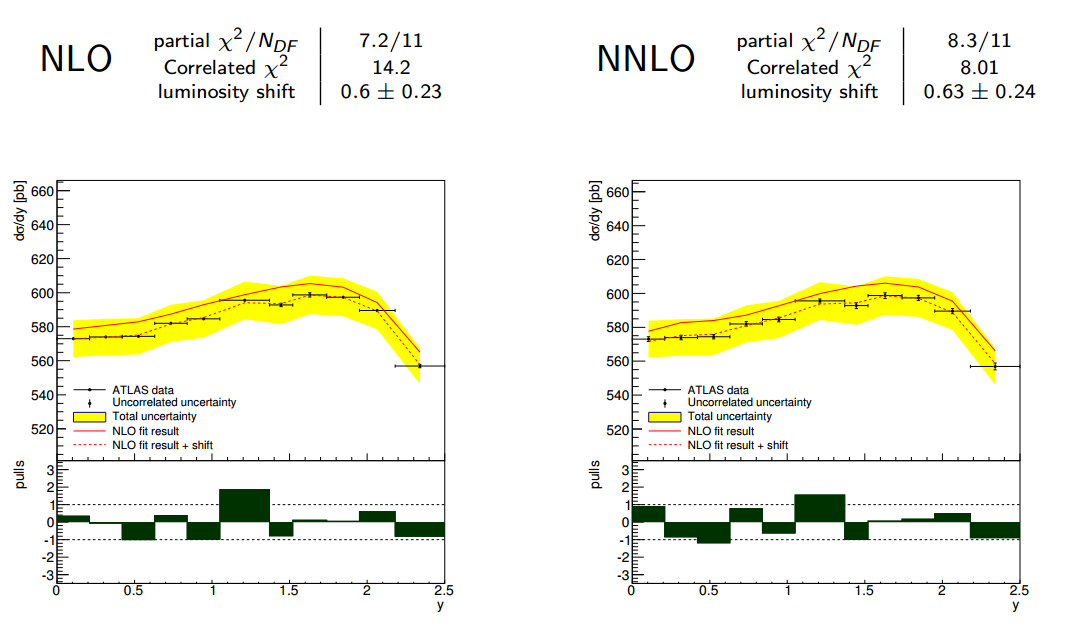
\includegraphics[width=0.9\textwidth]{dates/mtg/figures/wz/pdf_wplus}

\end{frame}

\begin{frame}{Fit with free $r_s$ to W,Z combined datasets}
\begin{itemize}
\item{$r_s = \frac{\bar{s}(x)}{\bar{d}(x)}$ \\
$\rightarrow$  $r_s \simeq 0.5$ (suppressed strangeness) is assumed in many PDFs}
\end{itemize}

\begin{columns}
\begin{column}{5cm}
\begin{itemize}
\item{NLO fit}
\end{itemize}
\begin{table}
\begin{center}
\begin{small}
\begin{tabular}[c]{c|c}
Z partial $\chi^2/N_{DF}$   &     $16.8/15$        \\
W+ partial $\chi^2/N_{DF}$   &     $8.8/11$        \\
W- partial $\chi^2/N_{DF}$   &     $15.9/11$        \\
Correlated $\chi^2$      &        29.1          \\
luminosity shift         &     $0.35 \pm  0.15$ \\
%$f_s$         &     \alert{$0.482 \pm  0.016$} \\
$r_s$         &     \alert{$0.942 \pm 0.060$} \\
\end{tabular}
\end{small}
\end{center}
\end{table}
\end{column}
\begin{column}{5cm}
\begin{itemize}
\item{NNLO fit}
\end{itemize}
\begin{table}
\begin{center}
\begin{small}
\begin{tabular}[c]{c|c}
Z partial $\chi^2/N_{DF}$   &     $14.6/15$        \\
W+ partial $\chi^2/N_{DF}$   &     $7.1/11$        \\
W- partial $\chi^2/N_{DF}$   &     $12.0/11$        \\
Correlated $\chi^2$      &        19.5          \\
luminosity shift         &     $0.70 \pm  0.16$ \\
%$f_s$         &     \alert{$0.504 \pm  0.014$} \\
$r_s$         &     \alert{$1.016 \pm 0.057$} \\
\end{tabular}
\end{small}
\end{center}
\end{table}
\end{column}
\end{columns}

\begin{itemize}
\item 2010 data showed first hint of enhanced strangeness:
\iteb
\item $r_s = 1.0 \pm 0.2$
\itee
\item This analysis confirms enhanced strangeness with much higher precision.
\end{itemize}


\end{frame}



\slide{ Plans }
{
\iteb
\item Today we held the ``First'' Ph.D. Committee Meeting
\item Two more meetings are necessary
\iteb
\item (2) ``Pre-Oral''
\item (3) Final ``Oral Examination'' (defense)
\itee
\item Measurement is largely complete, with a few items remaining:
\iteb
\item Larger MC samples in pipeline (to reduce systematics)
\item Double-differential combination and comparison with theory
\item Additional theory predictions and PDF fits
\item Various cross-checks and clarifications
\itee
\item What is everyone's availability over the summer?
\itee
}

%%%%%%% Back-up slides %%%%%%%%%%
\appendix
\newcounter{finalframe}
\setcounter{finalframe}{\value{framenumber}}

\slide{}
{
\centering
\Huge Back-up slides
}

\slide{Muon momentum scale: K}
{
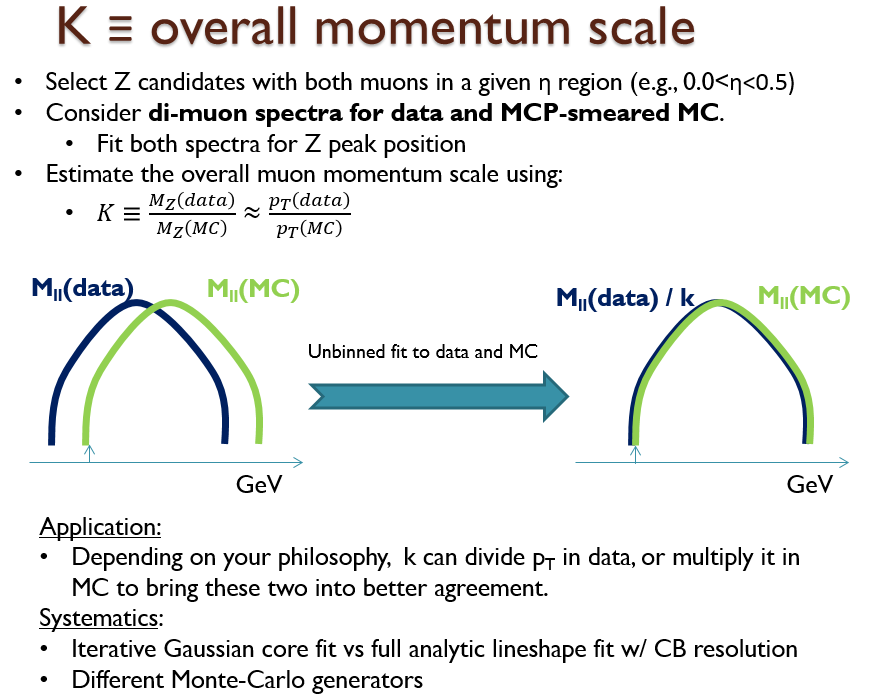
\includegraphics[width=0.8\textwidth]{dates/mtg/figures/mcp/K}
}
\slide{Muon momentum scale: C}
{
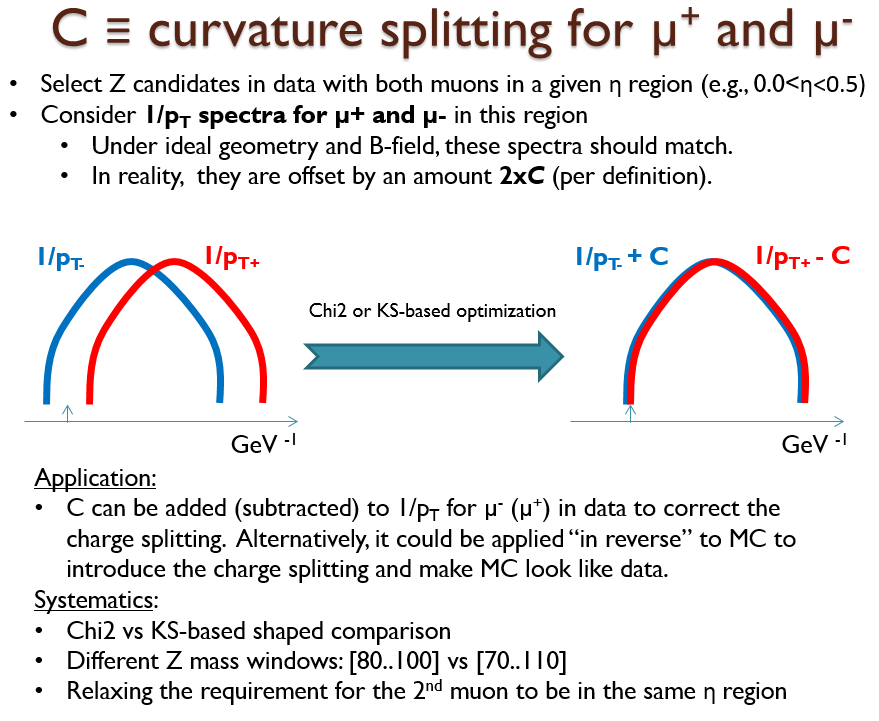
\includegraphics[width=0.8\textwidth]{dates/mtg/figures/mcp/C}
}

\input{/home/antonk/SupportingDocument/talk/fiducial_volumes.tex}
